\documentclass[../main.tex]{subfiles}

\begin{document}


    Testowanie oparte na \textbf{strukturze} oprogramowania lub systemu, np.:

    \begin{tabular}{p{4cm} | p{8cm}}
        \textbf{Poziom testów} & \textbf{Przykład struktury}\\
        \hline
        \textbf{testy modułowe} & kod: instrukcje, decyzje, rozgałęzienia, ścieżki\\
        \textbf{testy integracyjne} & drzewo wywołań\\
        \textbf{testy systemowe} & struktura menu, proces biznesowy, struktura strony www\\
    \end{tabular}


    Przykładowe metody wizualizacji struktury:
    \begin{itemize}
        \item graf przepływu sterowania (CFG, Control Flow Graph) lub danych
        \item model procesu biznesowego w BPML
        \item diagram aktywności (czynności) w UML
    \end{itemize}
    W technikach białoskrzynkowych przypadki testowe projektuje się tak, by
    pokrywały określone elementy modelu (krawędzie, decyzje, ścieżki itp.)

    Pokrycie (dla metod białoskrzynkowych) sprawdza jakość testów czarnoskrzynkowych; następnie techniki
    białoskrzynkowe dostarczają testów w celu zwiększenia tego pokrycia.


    \begin{figure}[H]
        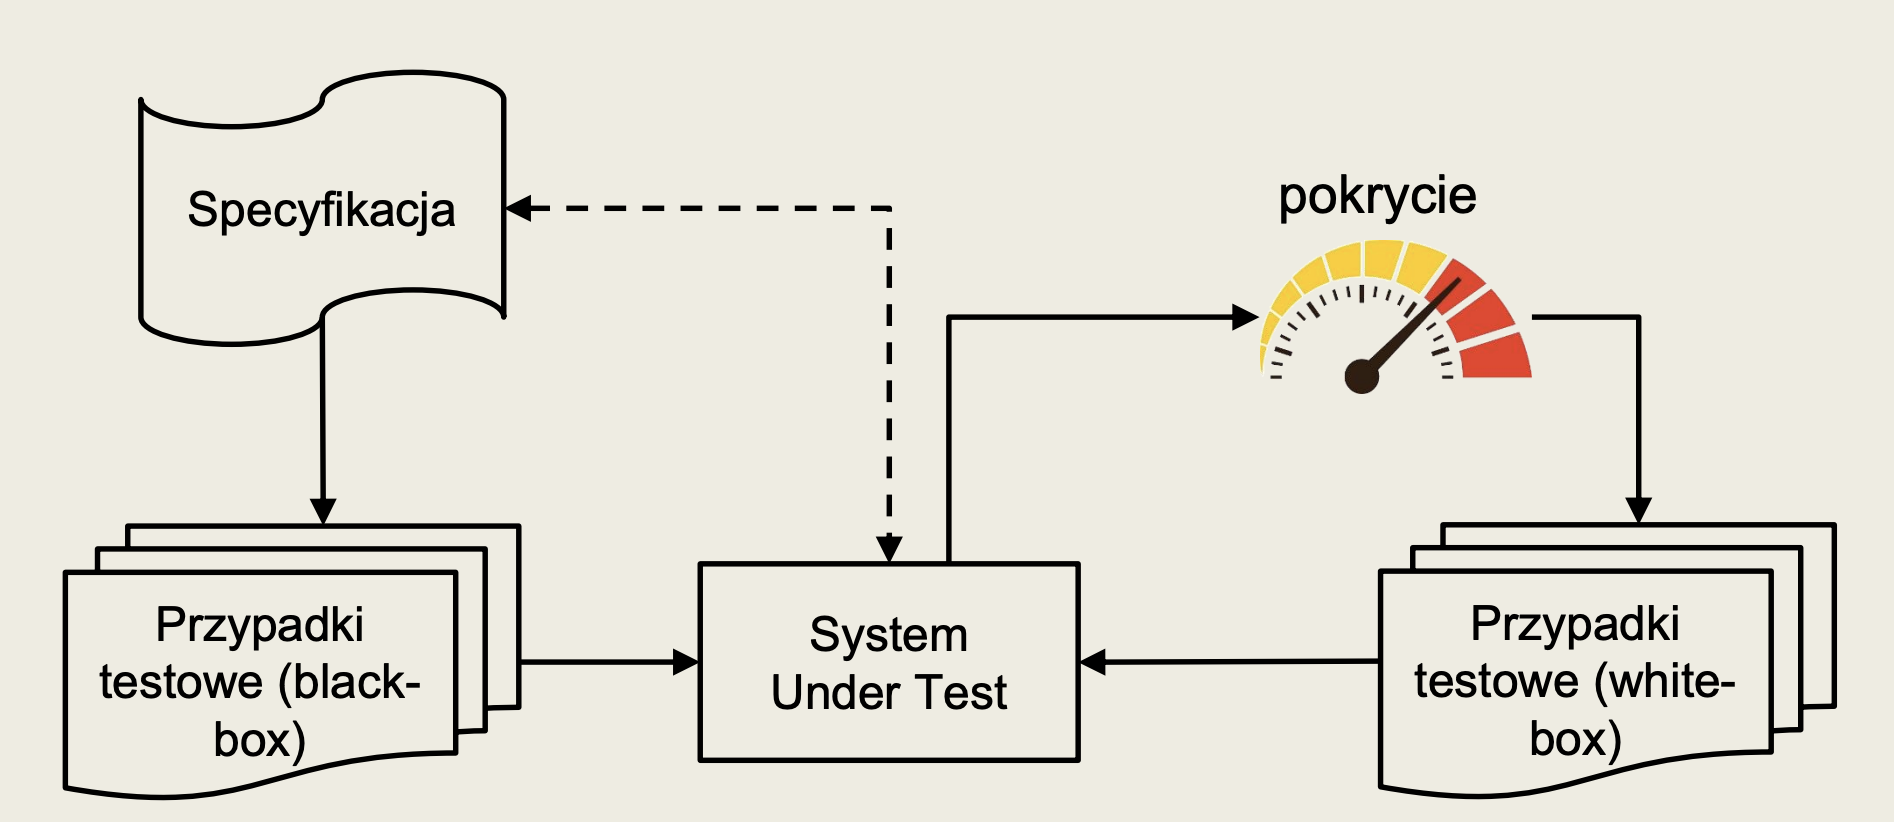
\includegraphics[width=\linewidth]{whitebox.png}
    \end{figure}


    \subsection{Pokrycia grafowe}

    \textbf{Pokrycie syntaktyczne i semantyczne}\\
    \textbf{Syntaktyczne} - "teoretyczne", wszystkie ścieżki grafu ignorując logikę poszczególnych węzłów.
    \textbf{Semantyczne} - uwzględniające tę logikę.

    \subsubsection{Graf przepływu sterowania}
    \begin{itemize}
        \item \textbf{CFG} - Control Flow Graph
        \item graficzna reprezentacja przepływu sterowania (graf skierowany)
        \begin{itemize}
            \item wierzchołki = bloki bazowe
            \item krawędzie = przejścia między blokami
        \end{itemize}
        \item blok bazowy = sekwencja instrukcji taka, że jeśli wykona się
        pierwsza z nich, wszystkie pozostałe w obrębie bloku wykonają się również
    \end{itemize}

    \begin{figure}[H]
        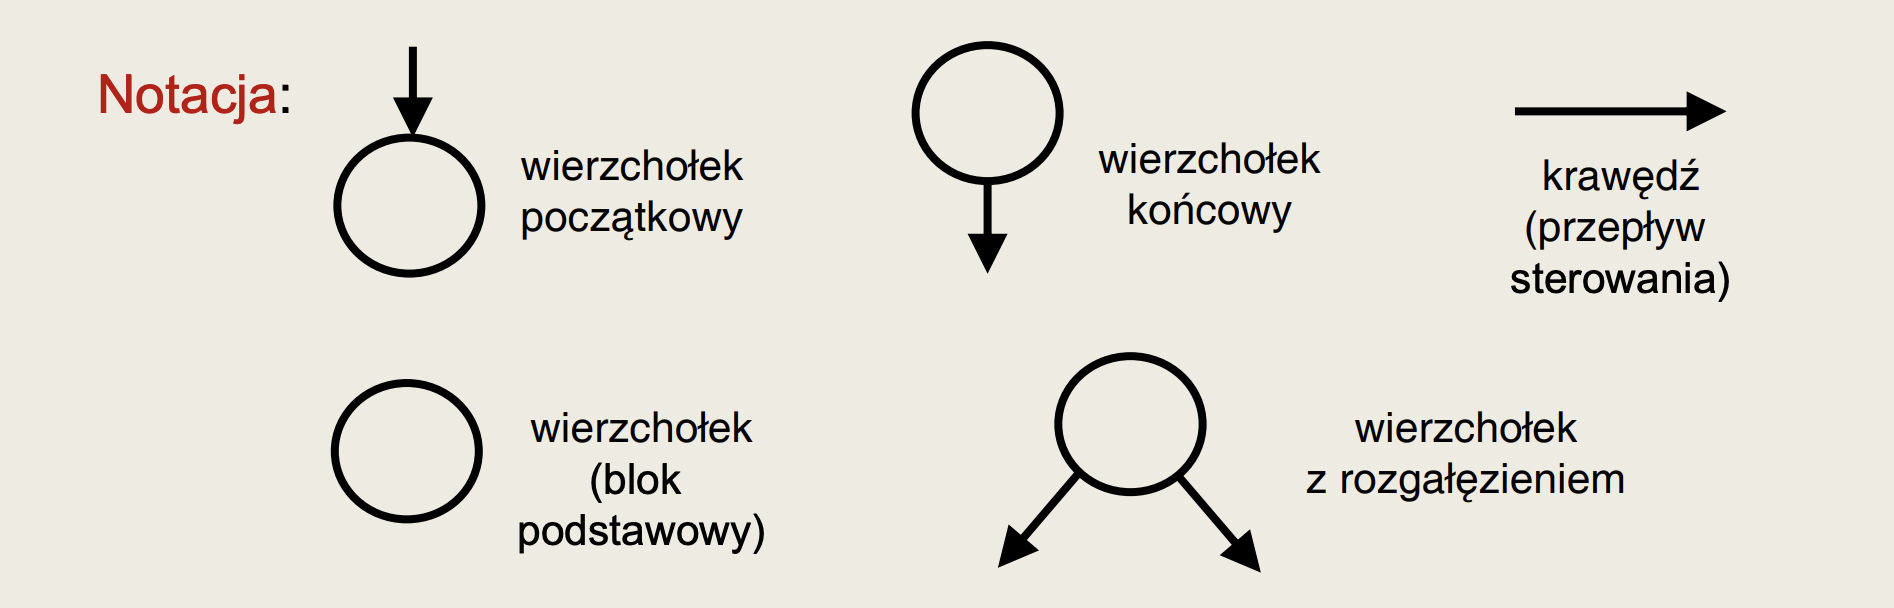
\includegraphics[width=\linewidth]{cfg.png}
    \end{figure}




    \subsubsection{Graf przepływu danych}
    \begin{itemize}
        \item oparty na grafie przepływ sterowania
        \item zawiera informacje o operacjach na zmiennych
        \item możliwe operacje:
        \begin{itemize}
            \item \textbf{d} (definition, definicja) – miejsce definiowania zmiennej
            \item \textbf{u} (use, użycie) – miejsce użycia zmiennej
            \item \textbf{k} (kill, zabicie) – miejsce usunięcia zmiennej z pamięci
        \end{itemize}
    \end{itemize}

    Dla każdego węzła $B$ definiujemy zbiory $d(B)$, $u(B)$, $k(B)$ zawierające zmienne definiowane, używane lub
    zabijane w danym węźle.

    \subsubsection{Pokrycia}

    \textbf{Pokrycie instrukcyjne}
    \begin{itemize}
        \item elementy pokrycia: instrukcje kodu
        \item kryterium pokrycia instrukcyjnego: każda linia kodu jest wykonana
        przynajmniej raz w jakimś teście
        \item pokrycie = liczba wykonanych instrukcji / liczba wszystkich instrukcji
        \item osiągnięcie 100\% pokrycia jest często nieosiągalne
    \end{itemize}
    Problemy praktyczne:
    \begin{itemize}
        \item jak definiować linię kodu? (linia fizyczna? wykonywalna?)
        \item czy rozważać pojedyncze instrukcje, czy bloki bazowe?
        \begin{itemize}
            \item to wpływa na metryki pokrycia
        \end{itemize}
    \end{itemize}


    \textbf{Pokrycie krawędziowe} (branch testing)
    \begin{itemize}
        \item inna nazwa: pokrycie przejść między instrukcjami
        \item z punktu widzenia struktury, wymagane jest przejście po każdej
        krawędzi CFG, czyli testowany jest każdy przepływ sterowania
        \item \textbf{suita testowa spełniająca 100\% pokrycia instrukcji nie musi
        spełniać 100\% przejść między instrukcjami!}
        \item Przy założeniu, że CFG ma co najmniej 1 krawędź, \textbf{pokrycie
        krawędziowe subsumuje pokrycie instrukcyjne, nie na odwrót}.
    \end{itemize}


    \textbf{Pełne pokrycie ścieżek}
    \begin{itemize}
        \item możliwe, gdy nie ma pętli lub liczba iteracji wszystkich pętli jest ograniczona z góry (rozsądną wartością)
        \item najczęstszy przypadek: diagramy przepływ procesów – zwykle nie zawierają pętli lub pętle są ograniczone
        \item nawet dla kodu bez pętli liczba wszystkich ścieżek może rosnąć wykładniczo względem punktów decyzyjnych
    \end{itemize}


    \textbf{Zbiór ścieżek liniowo niezależnych} to odpowiednik \textbf{bazy przestrzeni wektorowej}.\\
    \textbf{Złożoność cyklomatyczna CFG} - liczba ścieżek liniowo niezależnych.

    \textbf{Algorytm} wyznaczania ścieżek liniowo niezależnych:
    \begin{itemize}
        \item wychodzimy od prostej ścieżki
        \item jedna decyzja zmieniana w porównaniu z poprzednią ścieżką
        \item po zmianie, będąc w węźle już kiedyś odwiedzonym, kontynuujemy wędrówkę wzdłuż tamtej ścieżki,
        (staramy się zmienić tak mało, jak to możliwe, w porównaniu z poprzednimi ścieżkami)
        \item zwykle pętle iterujemy max. raz
    \end{itemize}



    \subsubsection{Pokrycie przepływu danych}
    \textbf{Ścieżka p z m do n jest def-czysta ze względu na zmienną v, jeśli v nie jest
    definiowana w żadnym węźle ścieżki p poza m.}


    Ścieżka $p = (p_1 , \dots, p_n)$ jest du-ścieżką ze względu na zmienną v, jeśli:
    \begin{enumerate}
        \item jest def-czysta ze względu na v
        \item $v \in def(p_1)$
        \item $v \in use(p_n)$
\end{enumerate}

    $du(n, v)$ - zbiór wszystkich du-ścieżek ze względu na v rozpoczynających się w n

    $du(n, m, v)$ - zbiór wszystkich du-ścieżek ze względu na v rozpoczynających się w n i kończących w m

    Kryteria pokrycia przepływu danych:
    \begin{itemize}
        \item \textbf{All-defs}: dla każdego wierzchołka n i definiowanej w nim zmiennej v
        zbiór testów zawiera przynajmniej jedną du-ścieżkę ze zbioru du(n, v)
        \item \textbf{All-uses}: dla każdej pary wierzchołków n, m i zmiennej v takich, że v jest
        definiowana w n i używana w m zbiór testów zawiera przynajmniej jedną
        du-ścieżkę ze zbioru du(n, m, v)
        \item \textbf{All-du-paths}: dla każdego wierzchołka n i definiowanej w nim zmiennej v
        zbiór testów zawiera wszystkie du-ścieżki ze zbioru du(n, v)
\end{itemize}

    \subsubsection{Pokrycie pętli}

    Co testujemy w przypadku pętli?
    \begin{itemize}
        \item problemy w inicjalizowaniu pętli (np. „błąd o jeden” w iteratorze)
        \item problemy z niezainicjalizowanymi zmiennymi (poprzez jednokrotne
        wykonanie pętli)
        \item problemy z powtarzaniem instrukcji zawartych w pętli
        \item kwestie związane z wydajnością/zasobami
    \end{itemize}

    Rodzaje pętli
    \begin{itemize}
        \item proste
        \begin{itemize}
            \item przetestuj brak wykonania pętli (pominięcie pętli, wykonanie 0 razy)
            \item przetestuj pojedyncze wykonanie pętli
            \item przetestuj podwójne wykonanie pętli
            \item przetestuj typową liczbę wykonań pętli
            \item przetestuj max-1, max, max+1 wykonań pętli, gdzie max =
            maksymalna dopuszczalna liczba iteracji
        \end{itemize}

        \item zagnieżdżone
        \begin{itemize}
            \item dla najbardziej zagnieżdżonej pętli przeprowadź test pętli prostej
            \item powtórz ten test dla kolejnych coraz bardziej zewnętrznych pętli
            \item powtarzaj, dopóki nie przetestujesz najbardziej zewnętrznej
        \end{itemize}

        \item połączone
        \begin{itemize}
            \item jeśli pętle połączone są niezależne, dla każdej z nich wykonaj test pętli prostej
            \item jeśli pętle połączone są zależne, przetestuj je jak zagnieżdżone
        \end{itemize}

        \item nieustrukturalizowane
        \begin{itemize}
            \item najlepsze wyjście: refaktoryzacja
            kodu w celu usunięcia
            nieustrukturyzowanych pętli
            \item pozbycie się instrukcji goto
        \end{itemize}
    \end{itemize}

    Problemy z testowaniem pętli
    \begin{itemize}
        \item istnienie pętli = nieskończona liczba ścieżek do przetestowania
        \item pętle zagnieżdżone = jeszcze większy problem
        \item defekty w pętlach są często trudne do wykrycia
        \item jak testować pętle? istnieją różne kryteria i podejścia
    \end{itemize}


\end{document}